\documentclass[12pt]{beamer}

\mode<presentation>
{
%   \usetheme[blue,noshadow]{Trondheim}
%   \usetheme[blue,minimal]{Trondheim}
  \usetheme[blue,compress,numbers,nonav,nologo]{Trondheim}
%   \usetheme[sand,compress,numbers,nonav,innovation]{Trondheim}
  % Some examples for the different options for beamerTrondheim

%   \usecolortheme{ntnuold}
  % try this if you encounter problems with the new ntnublue theme

  % \usefonttheme{professionalfonts}
  % Use only if using a font matching the conditions (see beamer docs)

  \usefonttheme[onlymath]{serif}
  % \useoutertheme{infolines}
  % or whatever

  \setbeamercovered{transparent}
  % or whatever (possibly just delete it)
}

\setbeamertemplate{blocks}[rounded][shadow=false]

% The following makes latex use nicer postscript fonts.
\usepackage{times}

% zorg dat het ganse document in sans-serif is
\renewcommand{\familydefault}{\sfdefault}

% Math support
\usepackage{amsmath}
\usepackage{amssymb}
\usepackage{amsfonts}
\usepackage{mathrsfs}

%found.
\usepackage{verbatim}

% put all math stuff in sans-serif
%\usepackage{sansmath}
%\sansmath

% Language support
%\usepackage[english]{babel}
\usepackage[dutch]{babel}

% Misc
%\usepackage[colorlinks,urlcolor=black,linkcolor=black,citecolor=black]{hyperref}
\usepackage{listings} % source listings
%\usepackage{multirow}
%\usepackage[times]{quotchap}
%\usepackage{setspace}

% Special words that latex has problem hyphenating.
\hyphenation{}

%\settaakheader
\title{What I learned from playing Kerbal Space Program}
\author{Niels Van Och \& Roeland Matthijssens}
\subject{Beamer}

\usepackage{graphicx}
\usepackage{moreverb}

\usepackage{latexsym}
\usepackage{indentfirst}
%\usepackage{amssymb}

\newcommand{\N}{\mathbb{N}}
\newcommand{\Z}{\mathbb{Z}}
\newcommand{\Q}{\mathbb{Q}}
\newcommand{\R}{\mathbb{R}}
\newcommand{\C}{\mathbb{C}}
\newcommand{\A}{\mathbb{A}}
\newcommand{\K}{\mathbb{K}}
\renewcommand{\H}{\mathbb{H}}
\renewcommand{\O}{\mathbb{O}}
\newcommand{\F}{\mathbb{F}}
\newcommand{\ltwee}{\mathnormal{l} ^2}

\newcommand{\dr}{\triangle}
\newcommand{\ring}{\C [\dr]}

\newcommand{\vect}{\mathrm{vect}}
\newcommand{\proj}{\mathrm{proj}}
\newcommand{\im}{\mathrm{Im}}
\newcommand{\ch}{\mathrm{char}}
\newcommand{\sig}{\mathrm{sig}}
\newcommand{\rang}{\mathrm{rang}}
\newcommand{\card}{\mathrm{card}}
\newcommand{\supR}{\mathrm{supR}}
\newcommand{\ann}{\mathrm{Ann}}

\definecolor{blurred}{rgb}{0.36,0.40,0.72}

\setbeamertemplate{frametitle}[default][rounded=false,shadow=false]
\setbeamertemplate{title page}[default][rounded=true]
\setbeamercolor{author}{fg=white}
\setbeamercolor{date}{fg=white}


\begin{document}
	\section{}
{
\usebackgroundtemplate{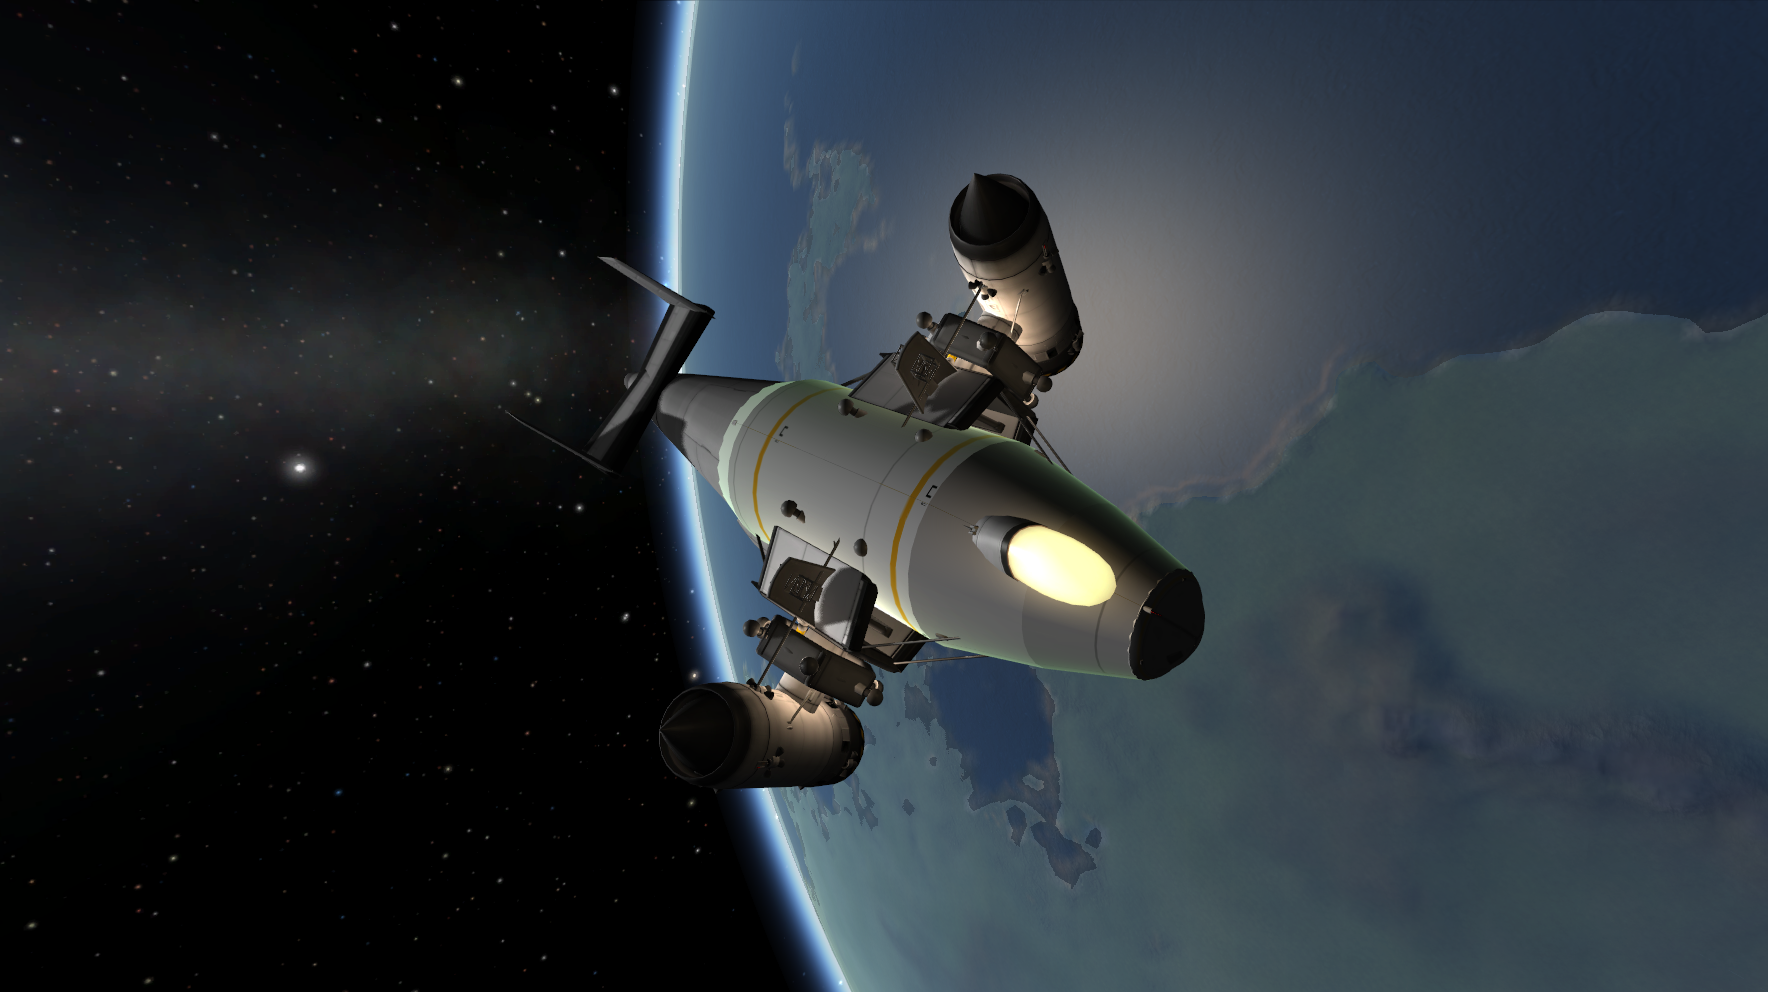
\includegraphics[height=\paperheight,keepaspectratio]{images/intro}}%
\begin{frame}
    \frametitle{Introduction}
    \begin{block}{}
        \begin{itemize}
            \item We'll take you through launching a rocket and landing it on a different planet
            \item Obviously: this is simplified
        \end{itemize}
    \end{block}
\end{frame}
\begin{frame}
    \frametitle{Technicalities}
    \begin{block}{Orbit}
        \begin{itemize}
            \item An object rotating around another object is said to be in orbit
        \end{itemize}
    \end{block}
\end{frame}
\begin{frame}
    \frametitle{Technicalities}
    \begin{block}{Delta-v}
        \begin{itemize}
            \item Your fuel budget
            \item How much can I accelerate/decelerate my rocket
            \item Depends on thrust to weight ratio
        \end{itemize}
    \end{block}
\end{frame}
}

{
\usebackgroundtemplate{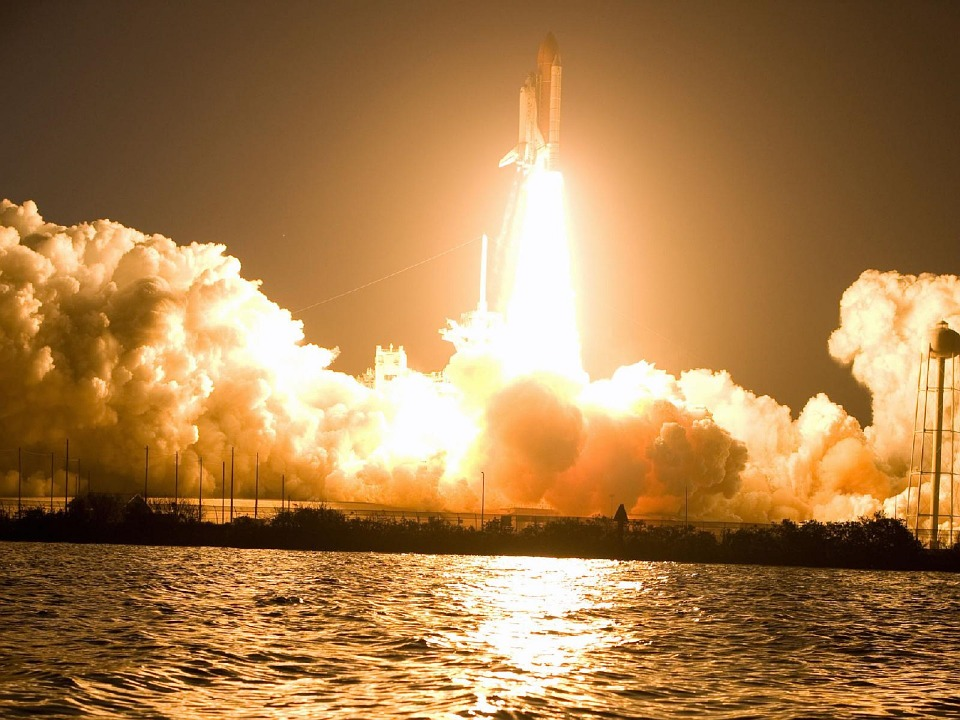
\includegraphics[height=\paperheight,keepaspectratio]{images/launch}}%
\begin{frame}
    \begin{block}{}
        \begin{center}
            Prepare for launch!
        \end{center}
    \end{block}
\end{frame}
}
{
\usebackgroundtemplate{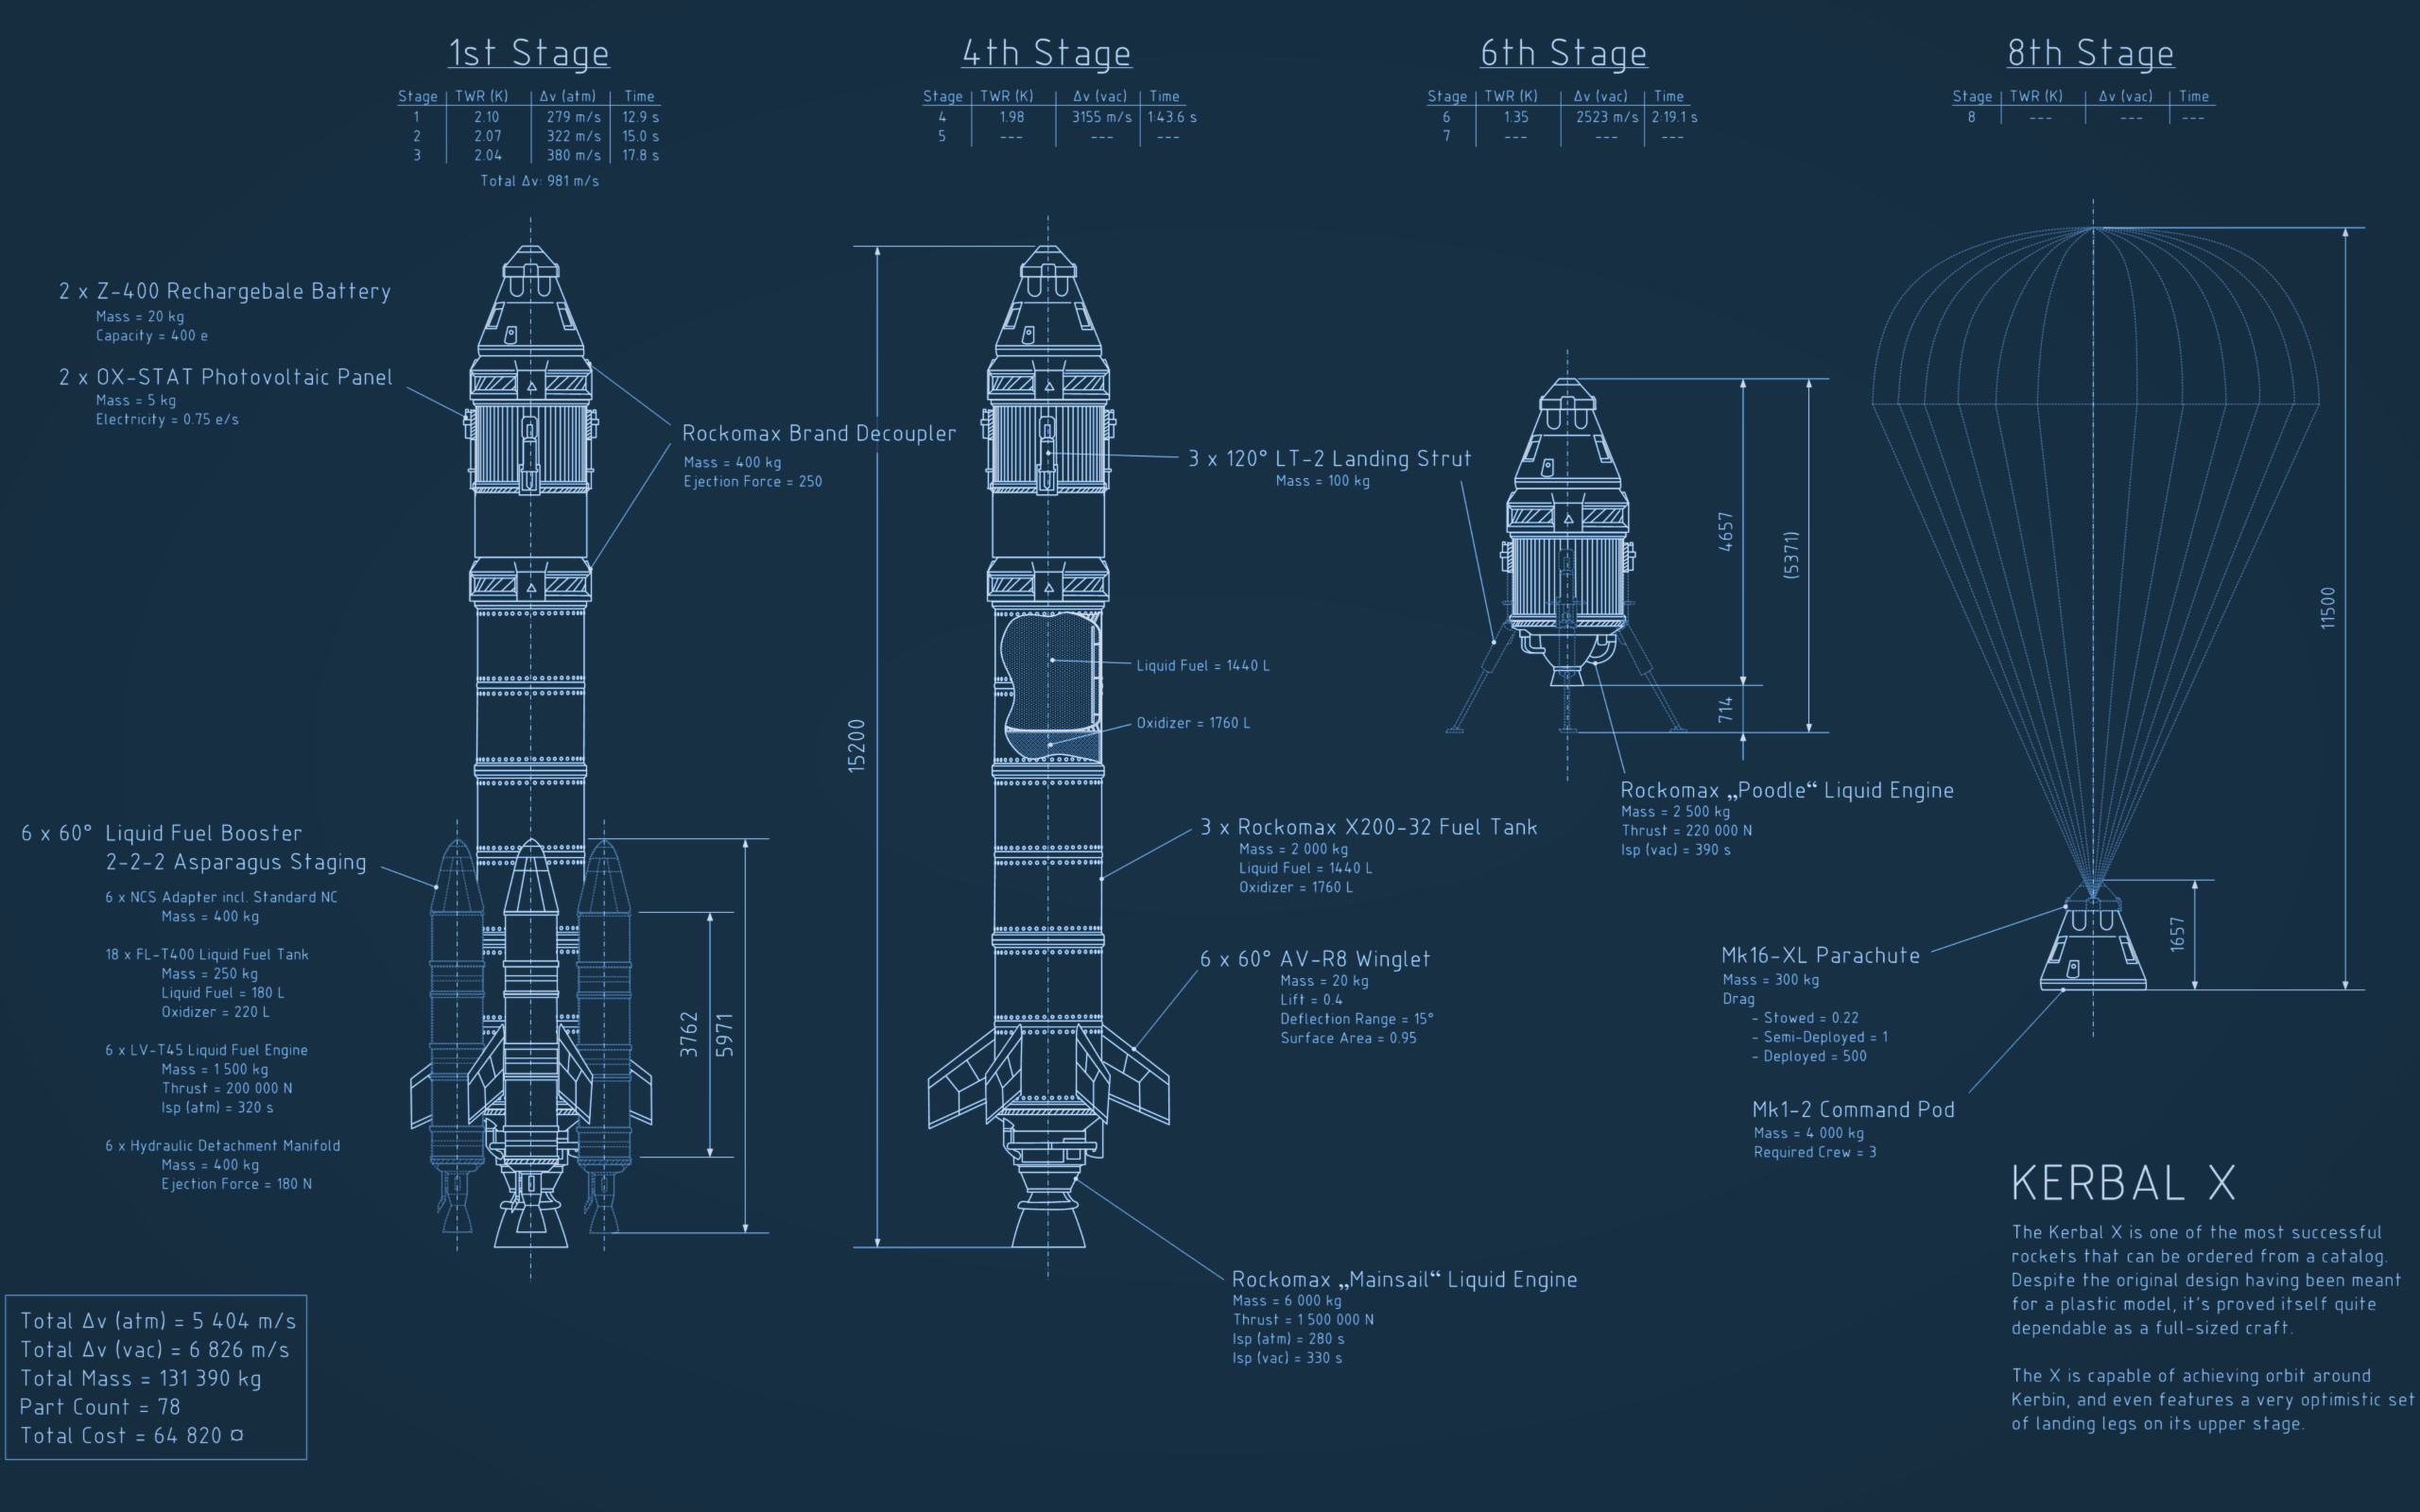
\includegraphics[height=\paperheight,keepaspectratio]{images/staging}}%
\begin{frame}
    \frametitle{Staging}
\end{frame}
\begin{frame}
    \frametitle{Staging}
    \begin{block}{How do we do it}
        \begin{itemize}
            \item Split the rocket in different parts (stages).
            \item Each stage carries its own fuel and engine, and can be separated from the rocket in sequence
            \item For instance: booster stage, transfer stage, landing stage, ...
        \end{itemize}
    \end{block}
\end{frame}
\begin{frame}
    \frametitle{Staging}
    \begin{block}{Why do we do it}
        \begin{itemize}
            \item Rocket efficiency is inversely proportional to its weight
            \item Delta-v goes up as total mass decreases, so we want to carry as little mass as posible
            \item Throw away excess weight of unused engines and empty fuel tanks
        \end{itemize}
    \end{block}
\end{frame}
}
\begin{frame}
    \frametitle{Staging}
    \begin{block}{}
        \begin{center}
            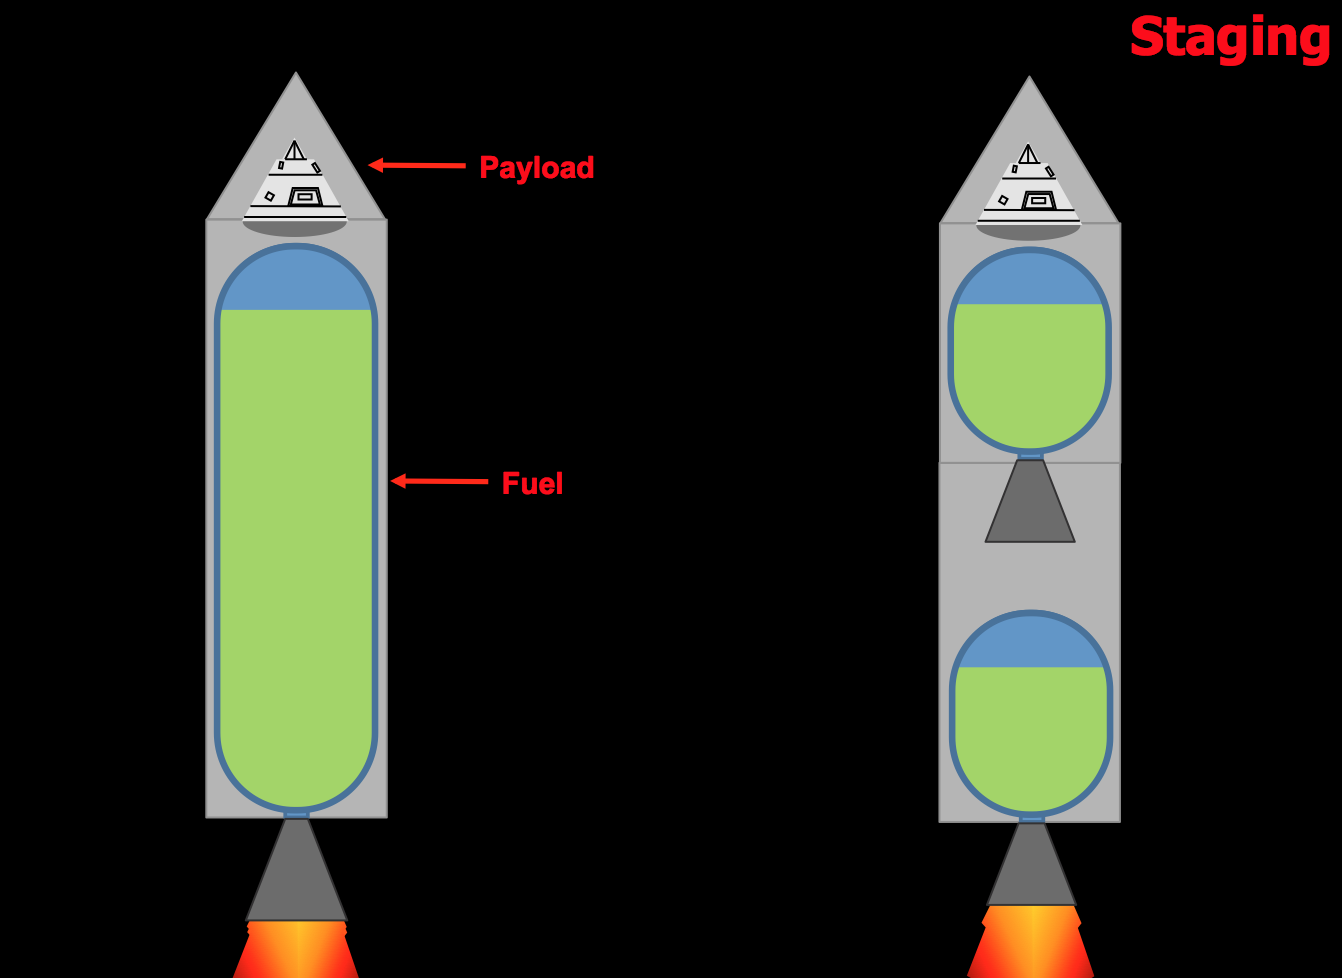
\includegraphics[width=0.5\textwidth]{images/staging1}
        \end{center}
    \end{block}
\end{frame}
\begin{frame}
    \frametitle{Staging}
    \begin{block}{}
        \begin{center}
            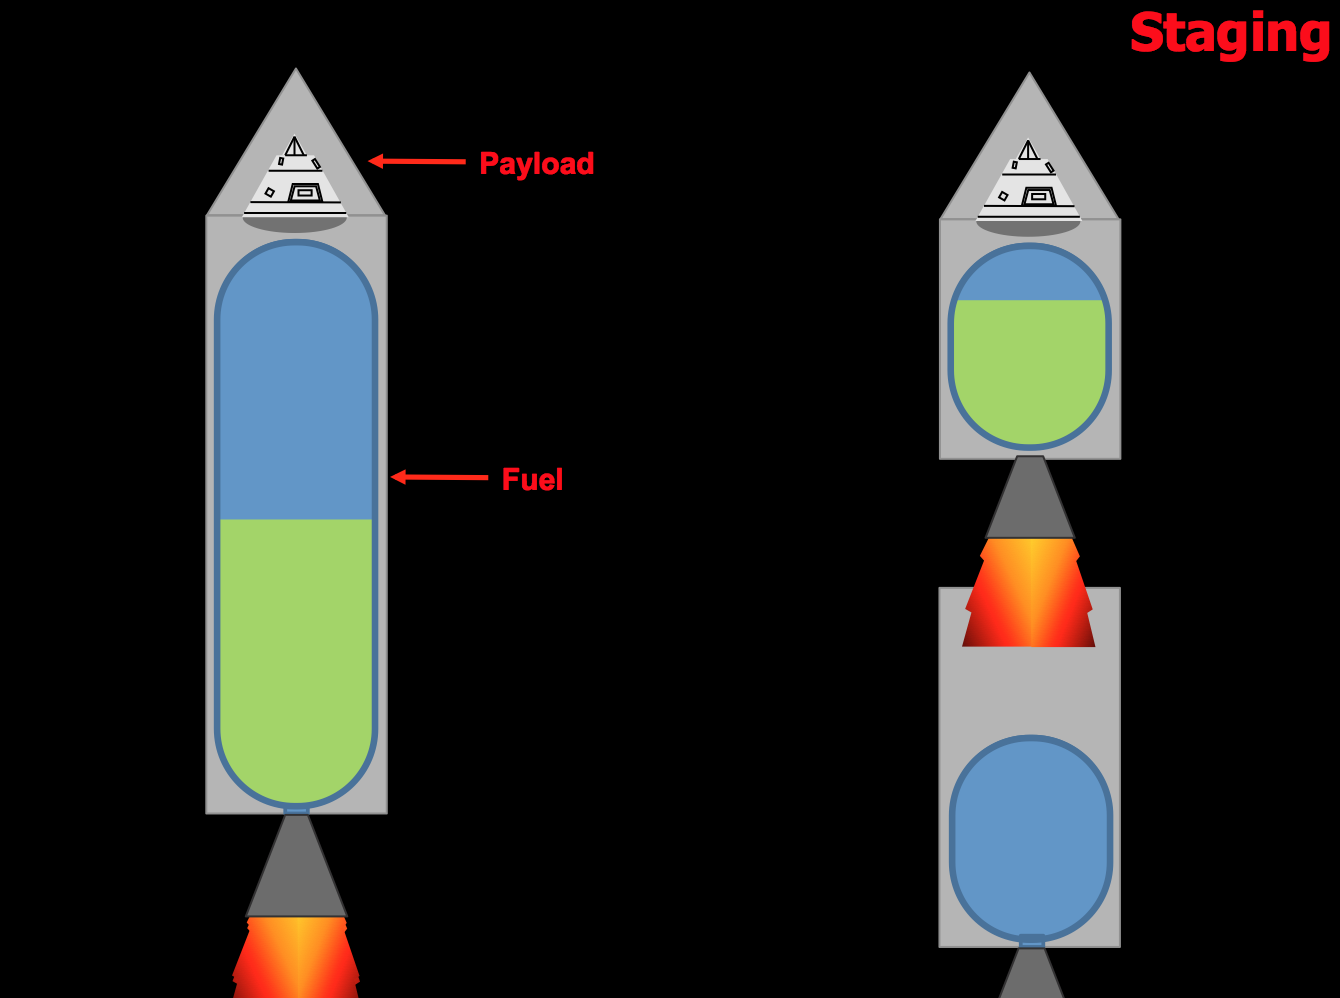
\includegraphics[width=0.5\textwidth]{images/staging2}
        \end{center}
    \end{block}
\end{frame}

{
\usebackgroundtemplate{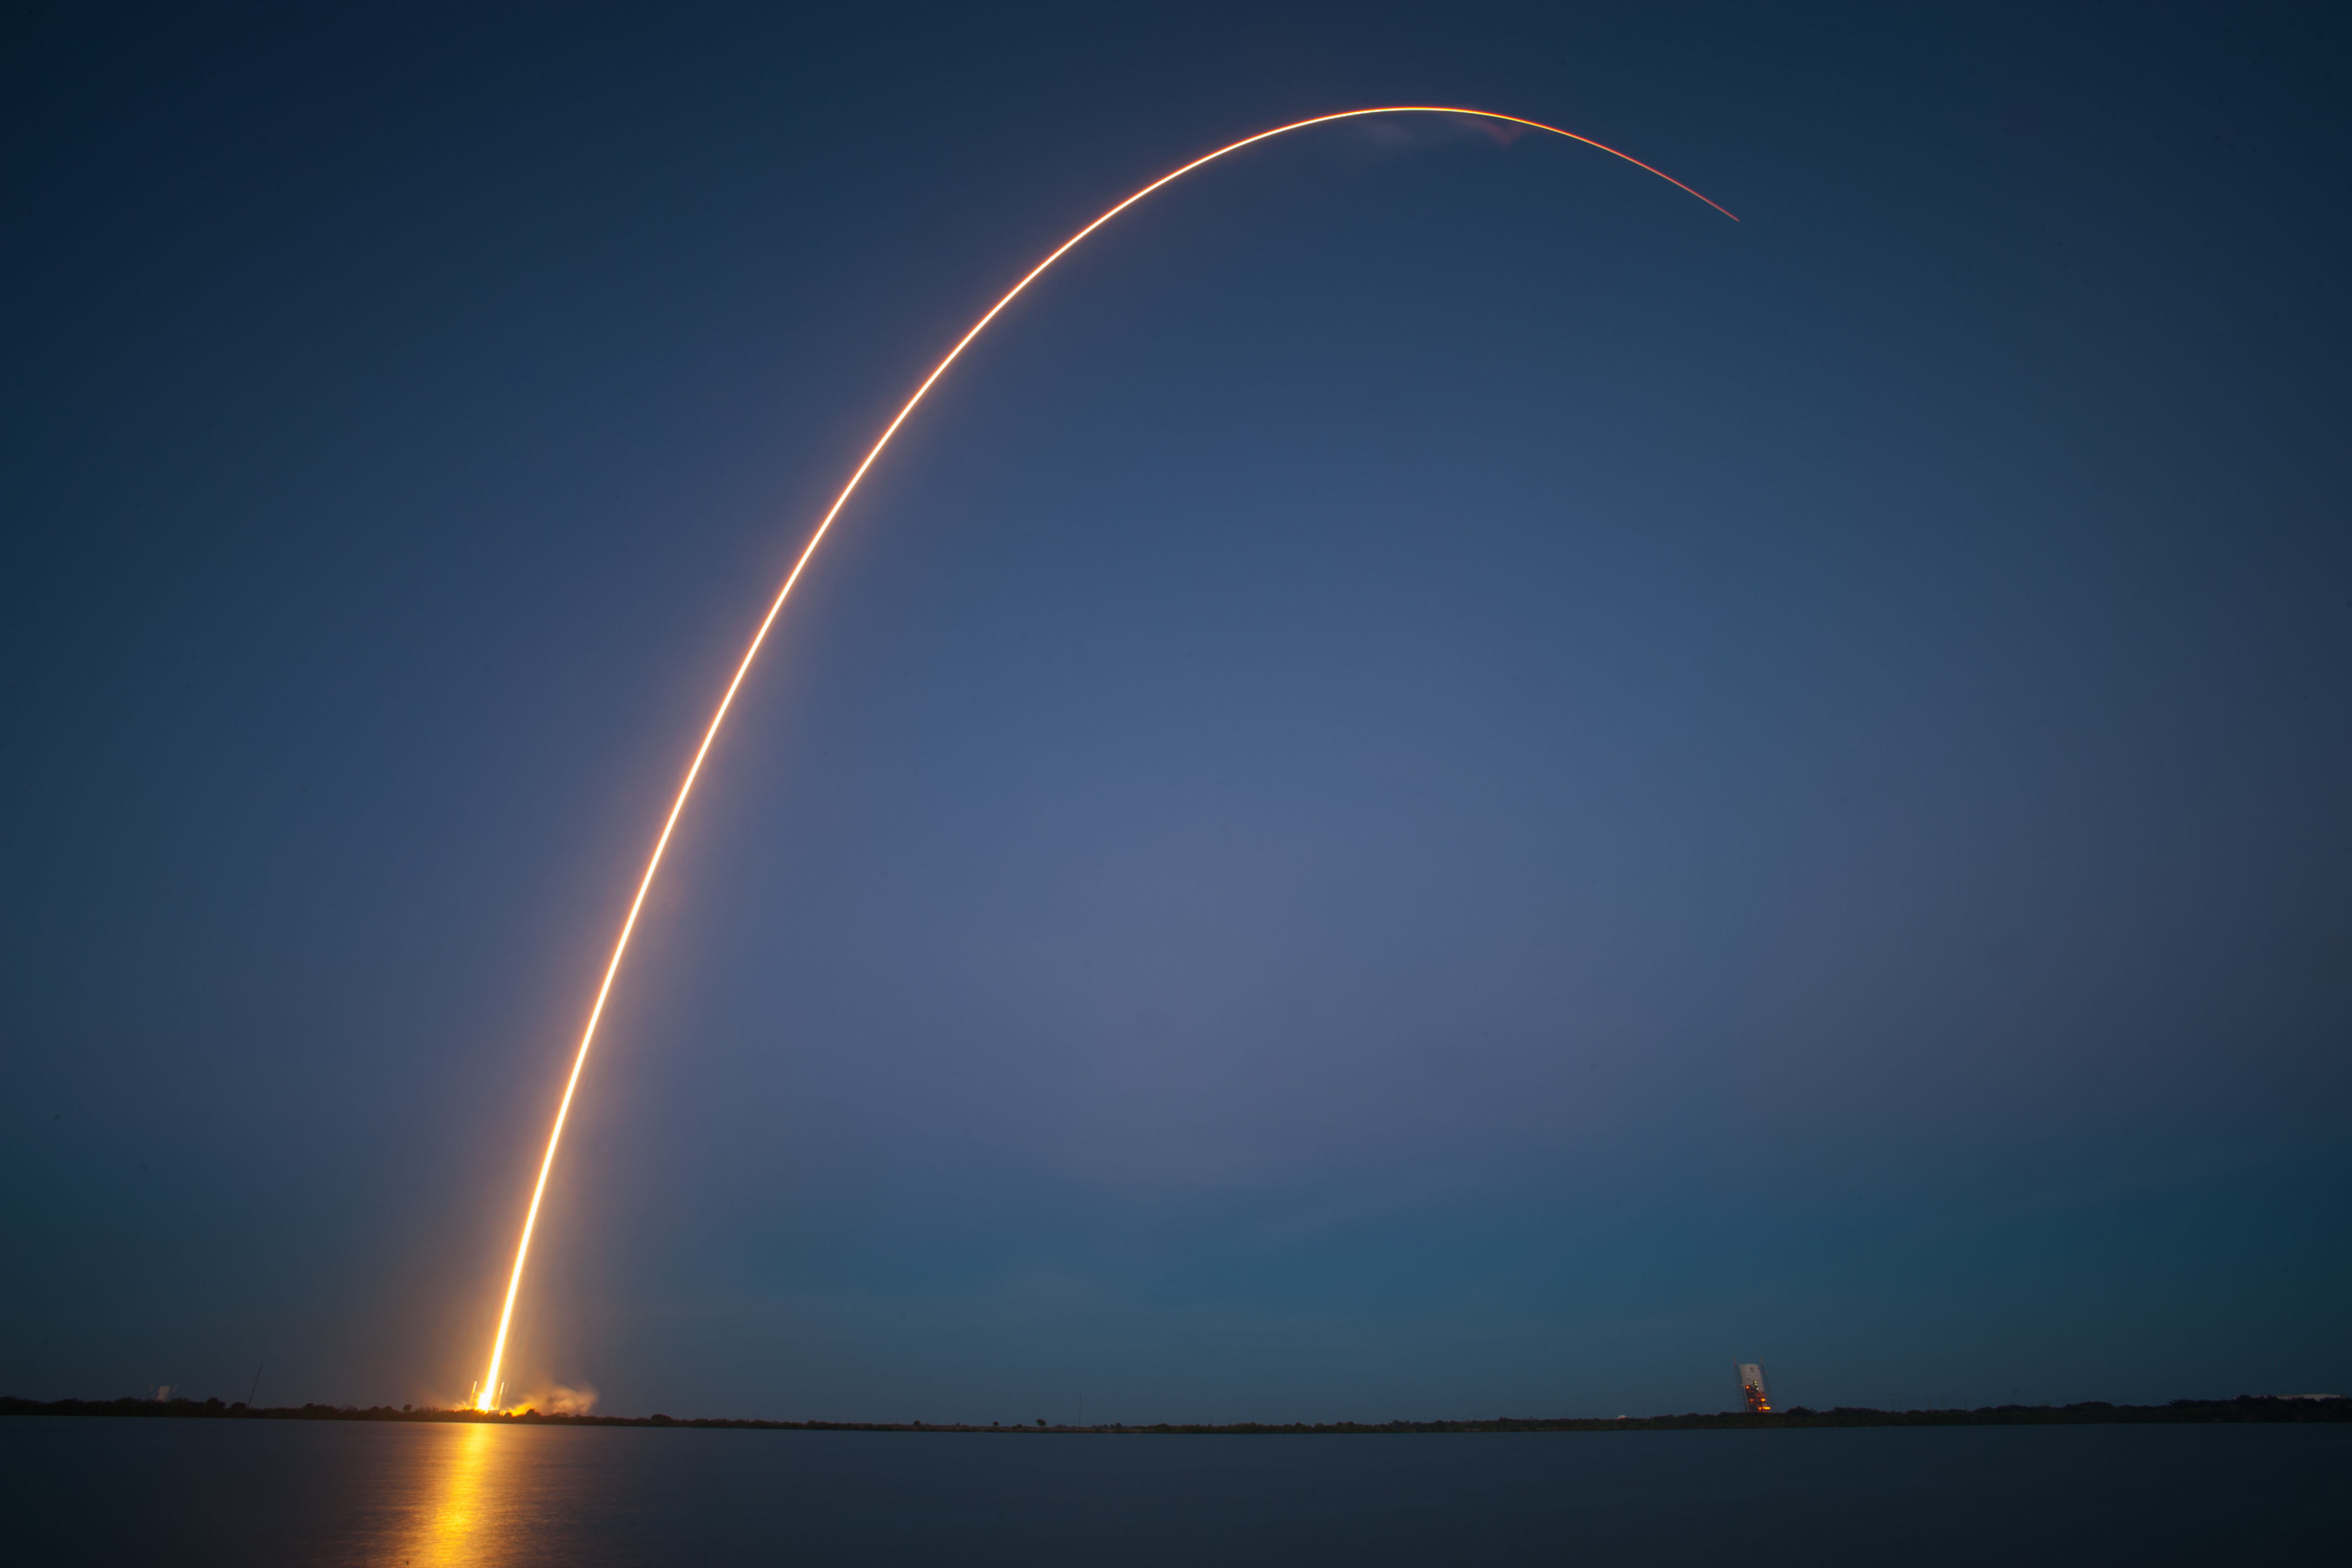
\includegraphics[height=\paperheight, keepaspectratio]{images/gravity_turn}}%
\begin{frame}
\end{frame}
\begin{frame}
    \frametitle{Getting into orbit}
    \begin{block}{Why do we turn?}
        \begin{itemize}
            \item Going straight up gains altitude quickly
            \item But we would just fall down again
            \item To get into orbit we need to move lateral as well
        \end{itemize}
    \end{block}
\end{frame}
\begin{frame}
    \frametitle{}
    \begin{block}{Gravity turn}
        \begin{itemize}
            \item Rotation of earth is already moving us towards the east at 1.5km/h. Turning east saves precious delta-v
            \item Rotational velocity is higher around the equator, so launch close to it (Cape Canaveral)
        \end{itemize}
    \end{block}
\end{frame}
\begin{frame}
    \frametitle{Let's launch!}
    \begin{block}{How do we do it?}
        \begin{itemize}
            \item Point eastward (about 5 degrees)
            \item Fire rocket
            \item Don't. Touch. Anything. Let gravity do the work
            \item Activate staging at the appropriate times
            \item Circularize orbit
            \item It's not rocket science
        \end{itemize}
    \end{block}
\end{frame}
}

{
\usebackgroundtemplate{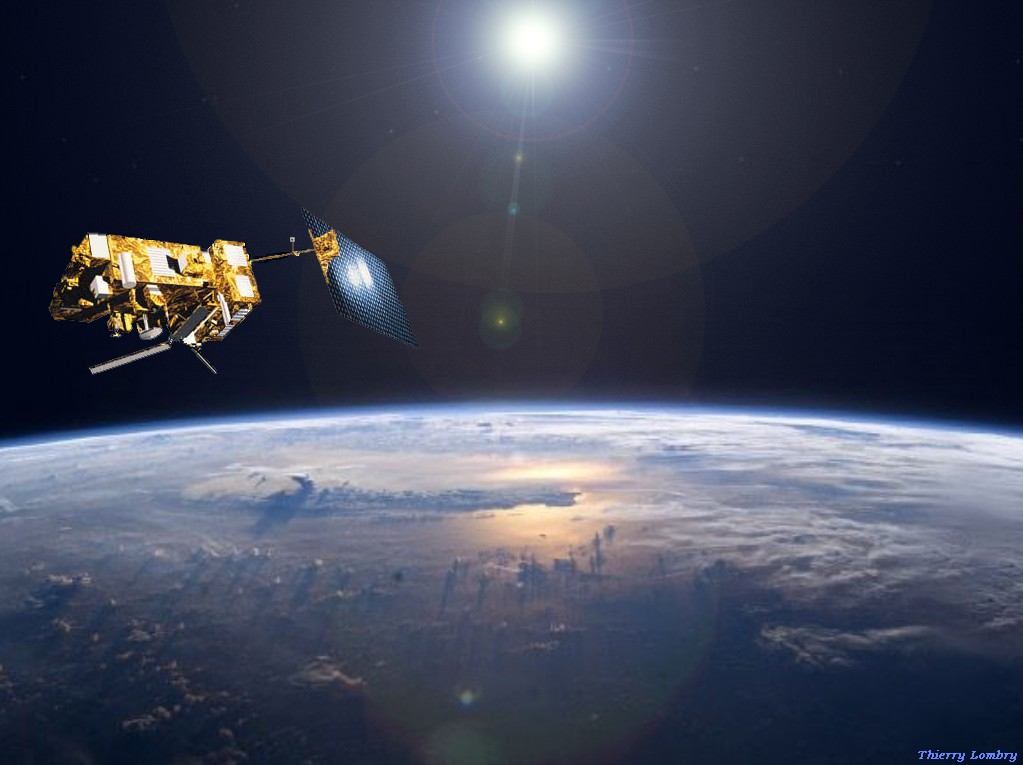
\includegraphics[height=\paperheight, keepaspectratio]{images/low_orbit}}%
\begin{frame}
\end{frame}
\begin{frame}
    \frametitle{About that circularizing}
    \begin{block}{}
        We are now almost in low earth orbit but still falling down. Our orbit could still cross the atmosphere.
        So we need to learn how to manipulate our orbit while in space.
    \end{block}
    \begin{block}{Basics}
        Movement on an orbit generally affects the opposite side of the orbit.
    \end{block}
\end{frame}
\begin{frame}
    \frametitle{Adjusting orbits}
    \begin{block}{}
        \begin{center}
            At any point on the orbit you can burn in 3 directions: up/down, left/right, forwards/backwards
        \end{center}
    \end{block}
    \begin{block}{}
        \begin{center}
            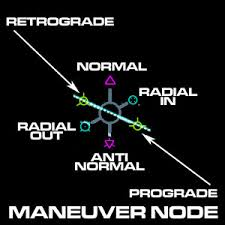
\includegraphics[scale=0.4]{images/maneuver_node}
        \end{center}
    \end{block}
\end{frame}
}

\begin{frame}
    \frametitle{Prograde}
    \begin{center}
        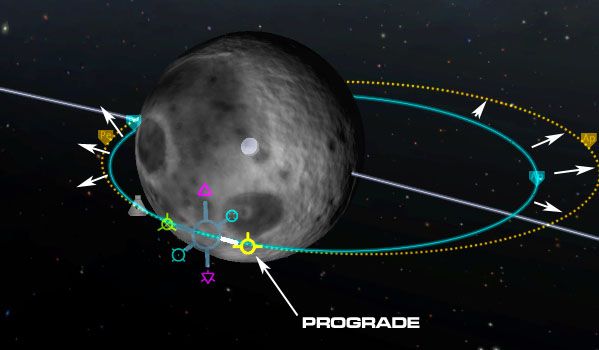
\includegraphics[scale=0.4]{images/prograde}
    \end{center}
\end{frame}
\begin{frame}
    \frametitle{Retrograde}
    \begin{center}
        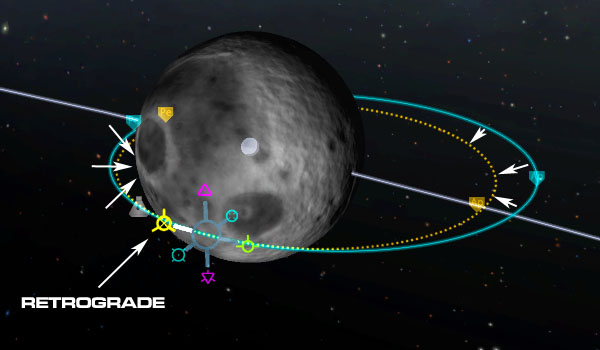
\includegraphics[scale=0.5]{images/retrograde}
    \end{center}
\end{frame}
\begin{frame}
    \frametitle{Normal}
    \begin{center}
        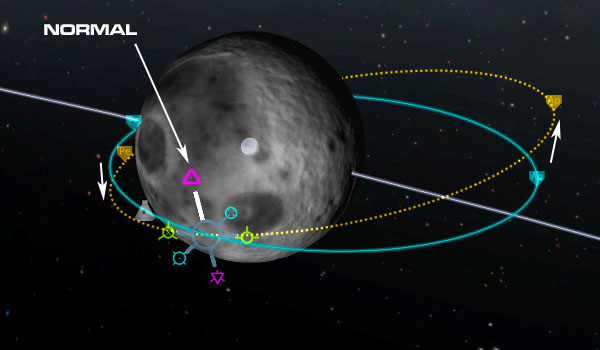
\includegraphics[scale=0.5]{images/normal}
    \end{center}
\end{frame}
\begin{frame}
    \frametitle{Anti-normal}
    \begin{center}
        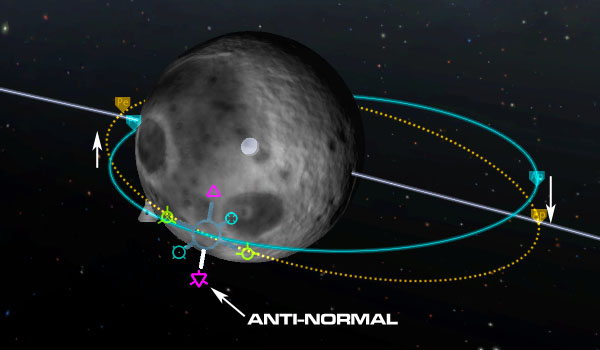
\includegraphics[scale=0.4]{images/anti_normal}
    \end{center}
\end{frame}
\begin{frame}
    \begin{center}
        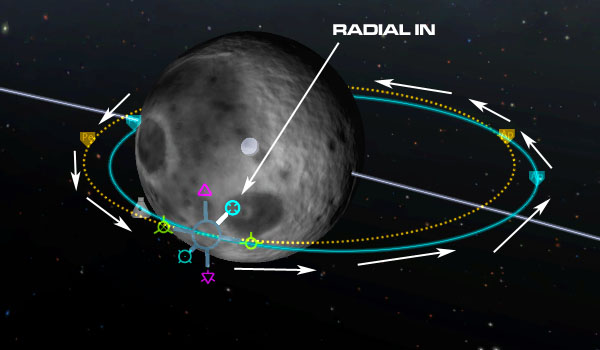
\includegraphics[scale=0.5]{images/radial_in}
    \end{center}
\end{frame}
\begin{frame}
    \frametitle{Radial out}
    \begin{center}
        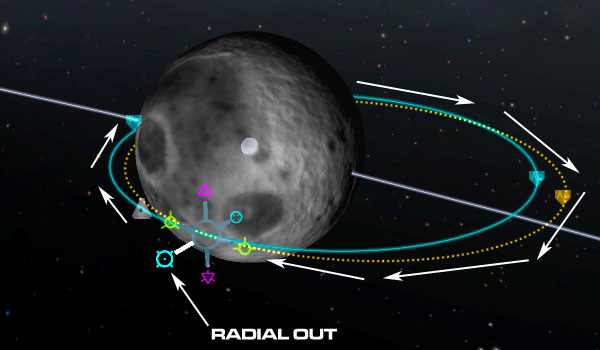
\includegraphics[scale=0.5]{images/radial_out}
    \end{center}
\end{frame}

\begin{frame}
    \frametitle{Planning transfer}
    \begin{block}{}
        We finally achieved a stable low earth orbit. We need to plan our transfer to our target body
    \end{block}
\end{frame}
\begin{frame}
    \begin{center}
        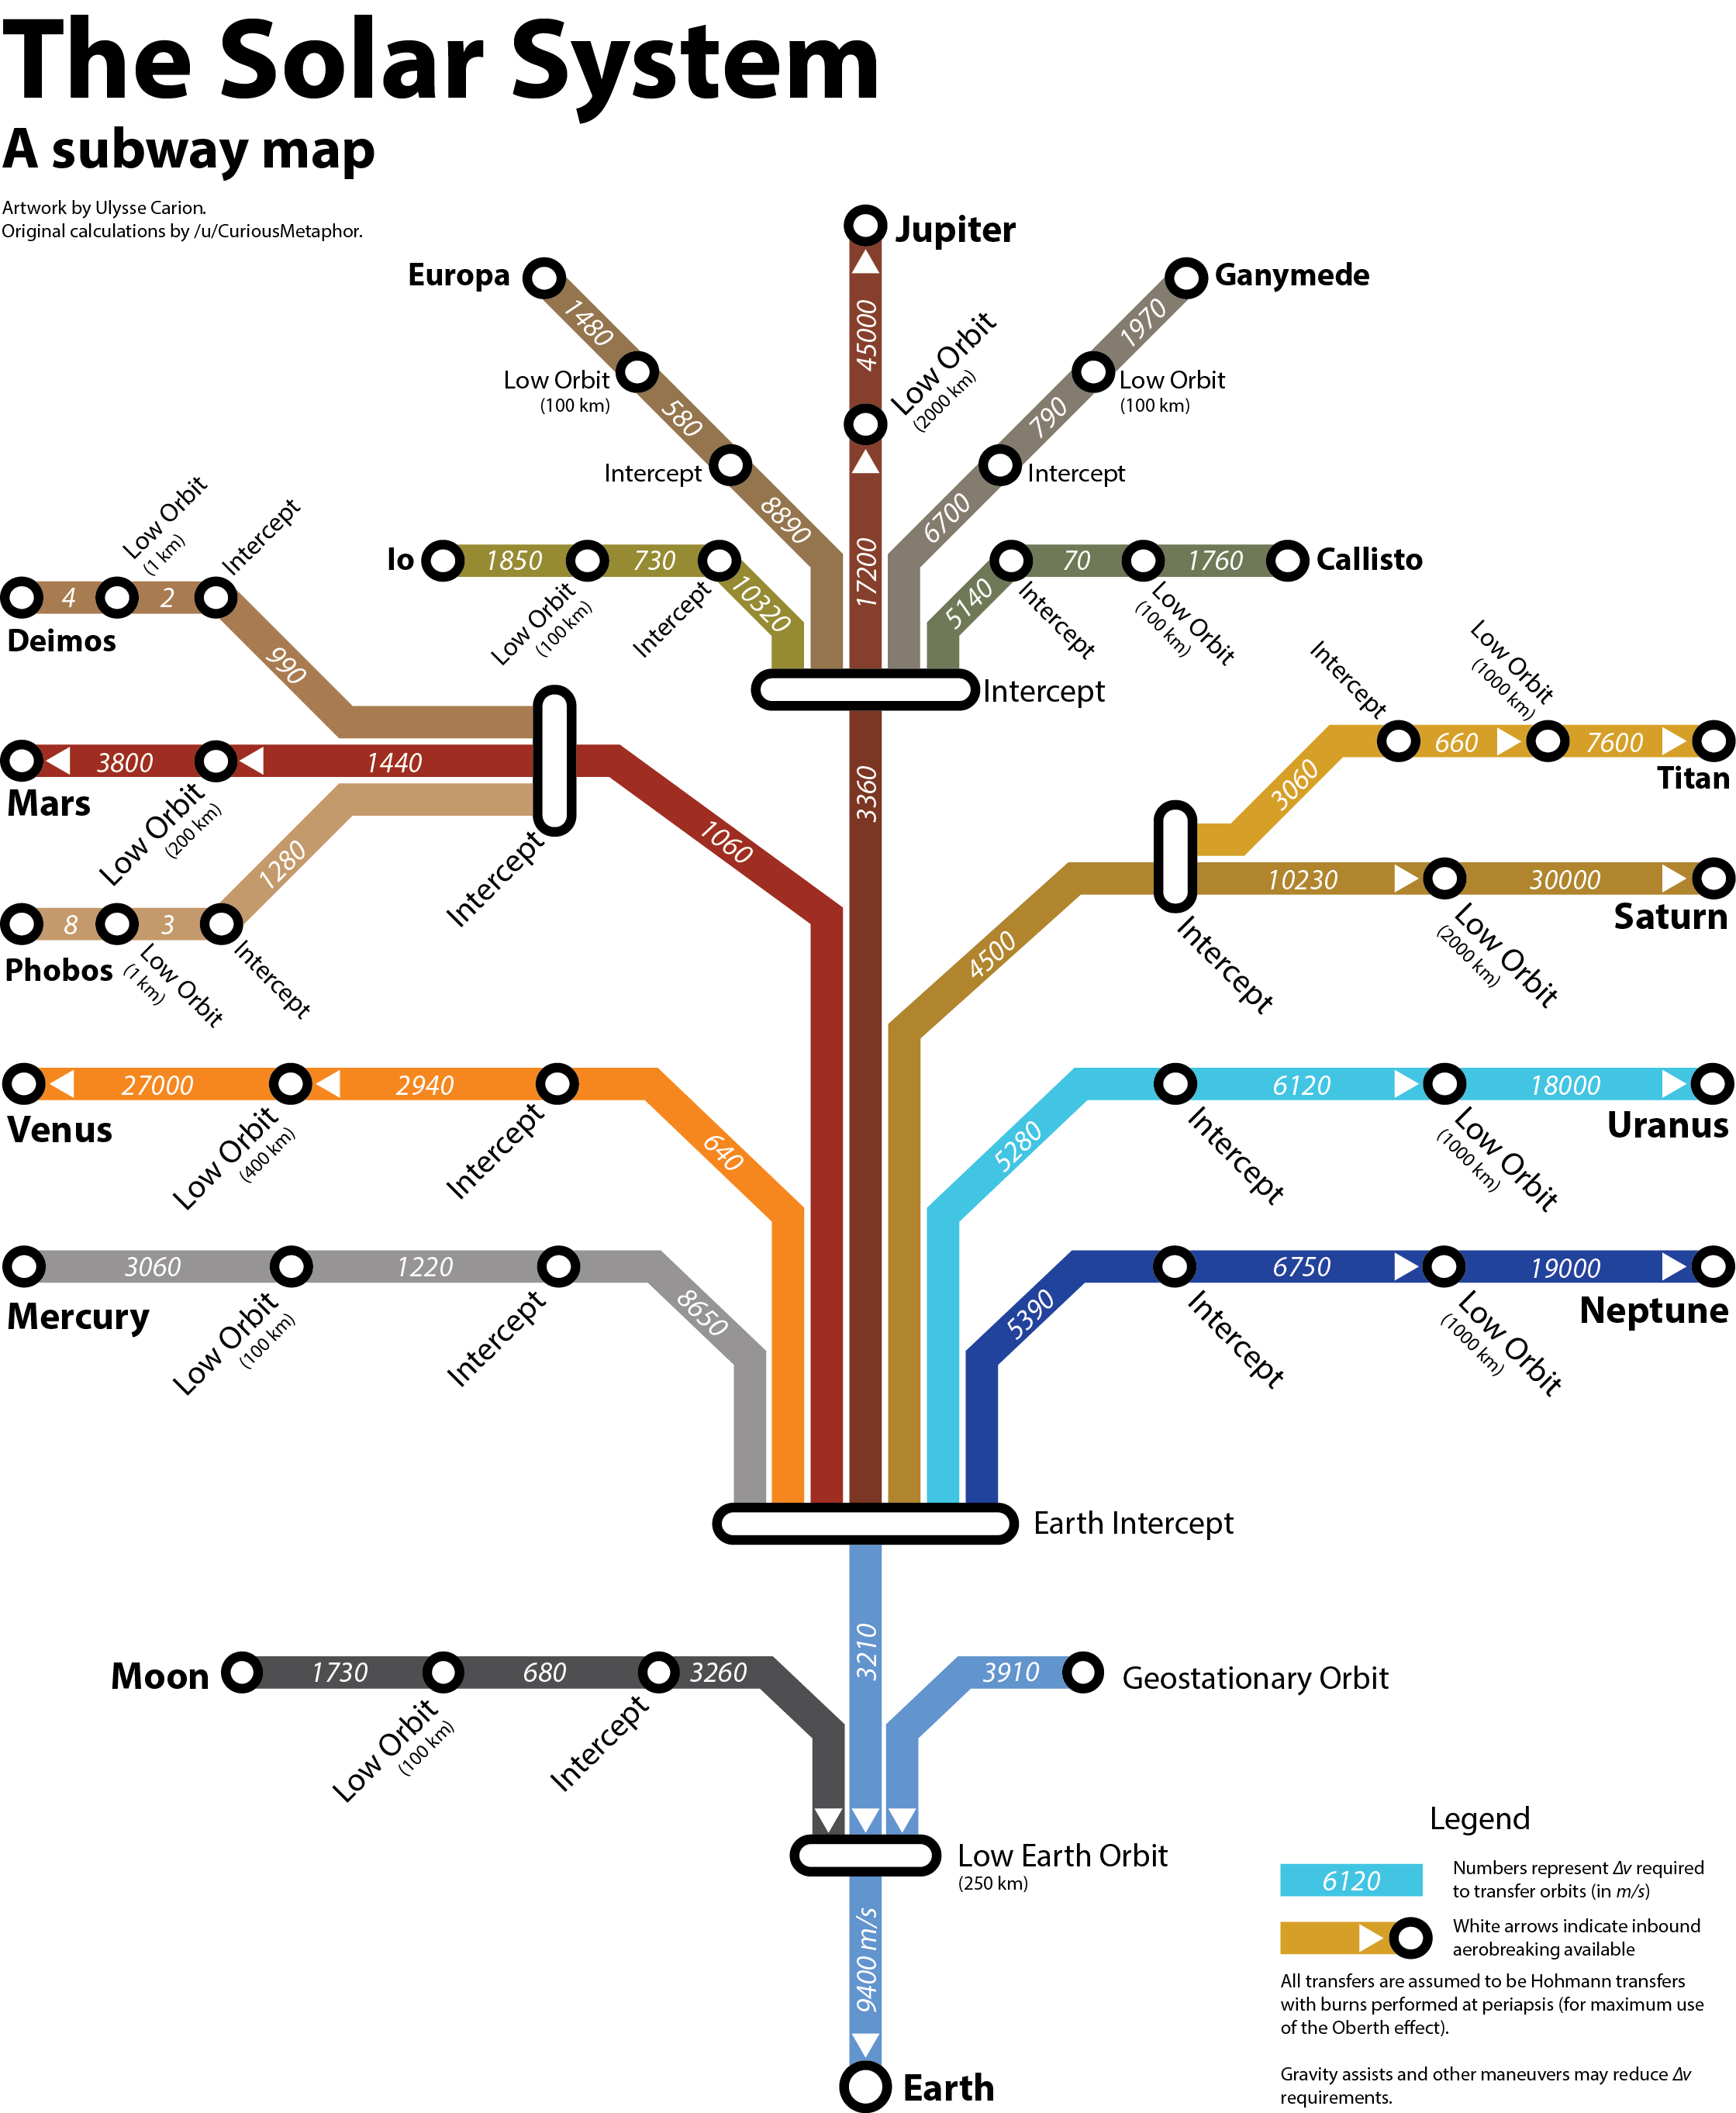
\includegraphics[height=\textheight]{images/deltavmap}
    \end{center}
\end{frame}
\begin{frame}
    \frametitle{Hohmann transfer}
    \begin{block}{}
        Now that we know our target and know the delta-v required to get there we need to plan the encounter
    \end{block}
    \begin{block}{}
        \begin{center}
            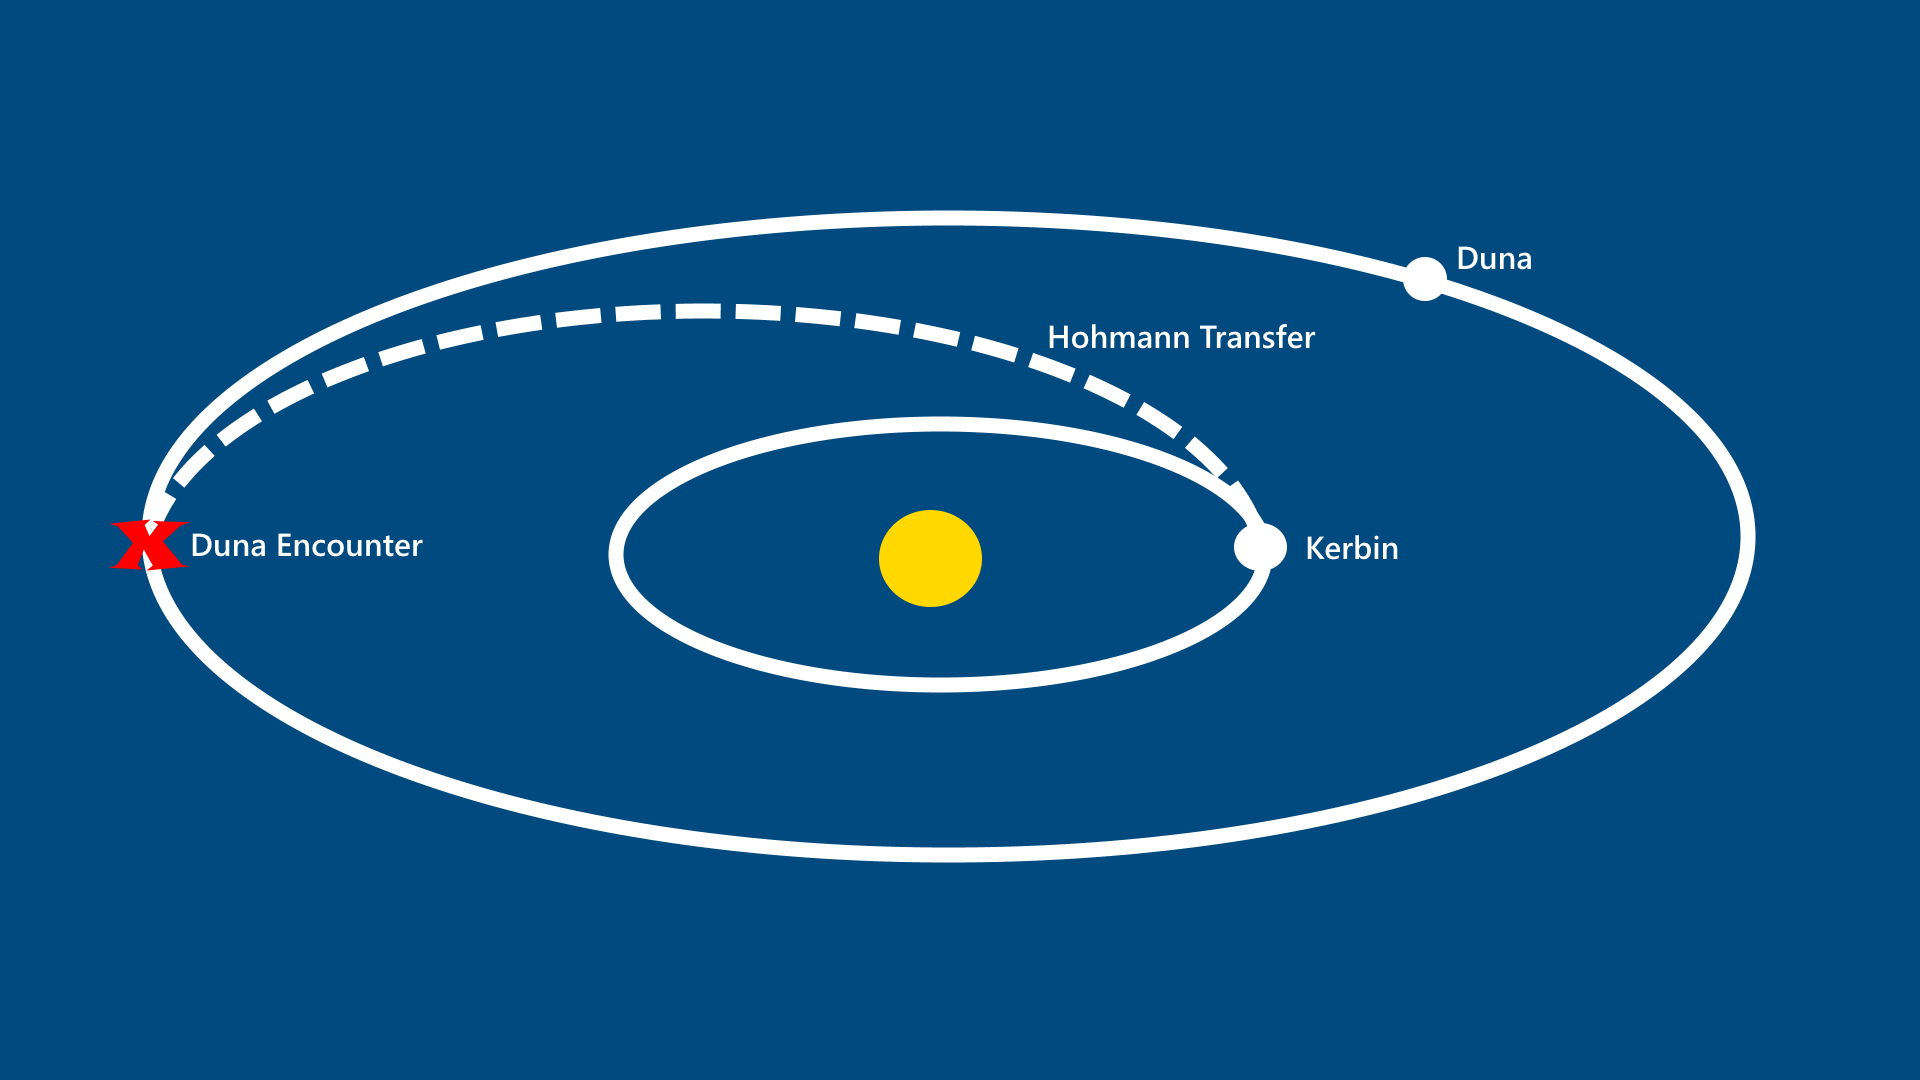
\includegraphics[scale=0.2]{images/hohmann_transfer}
        \end{center}
    \end{block}
\end{frame}
\begin{frame}
    \frametitle{Hohmann transfer window}
    \begin{block}{}
        To be able to transfer with the least amount of delta-v possible, we need to launch when the target body is
        at an optimal position
    \end{block}
    \begin{block}{}
        \begin{center}
            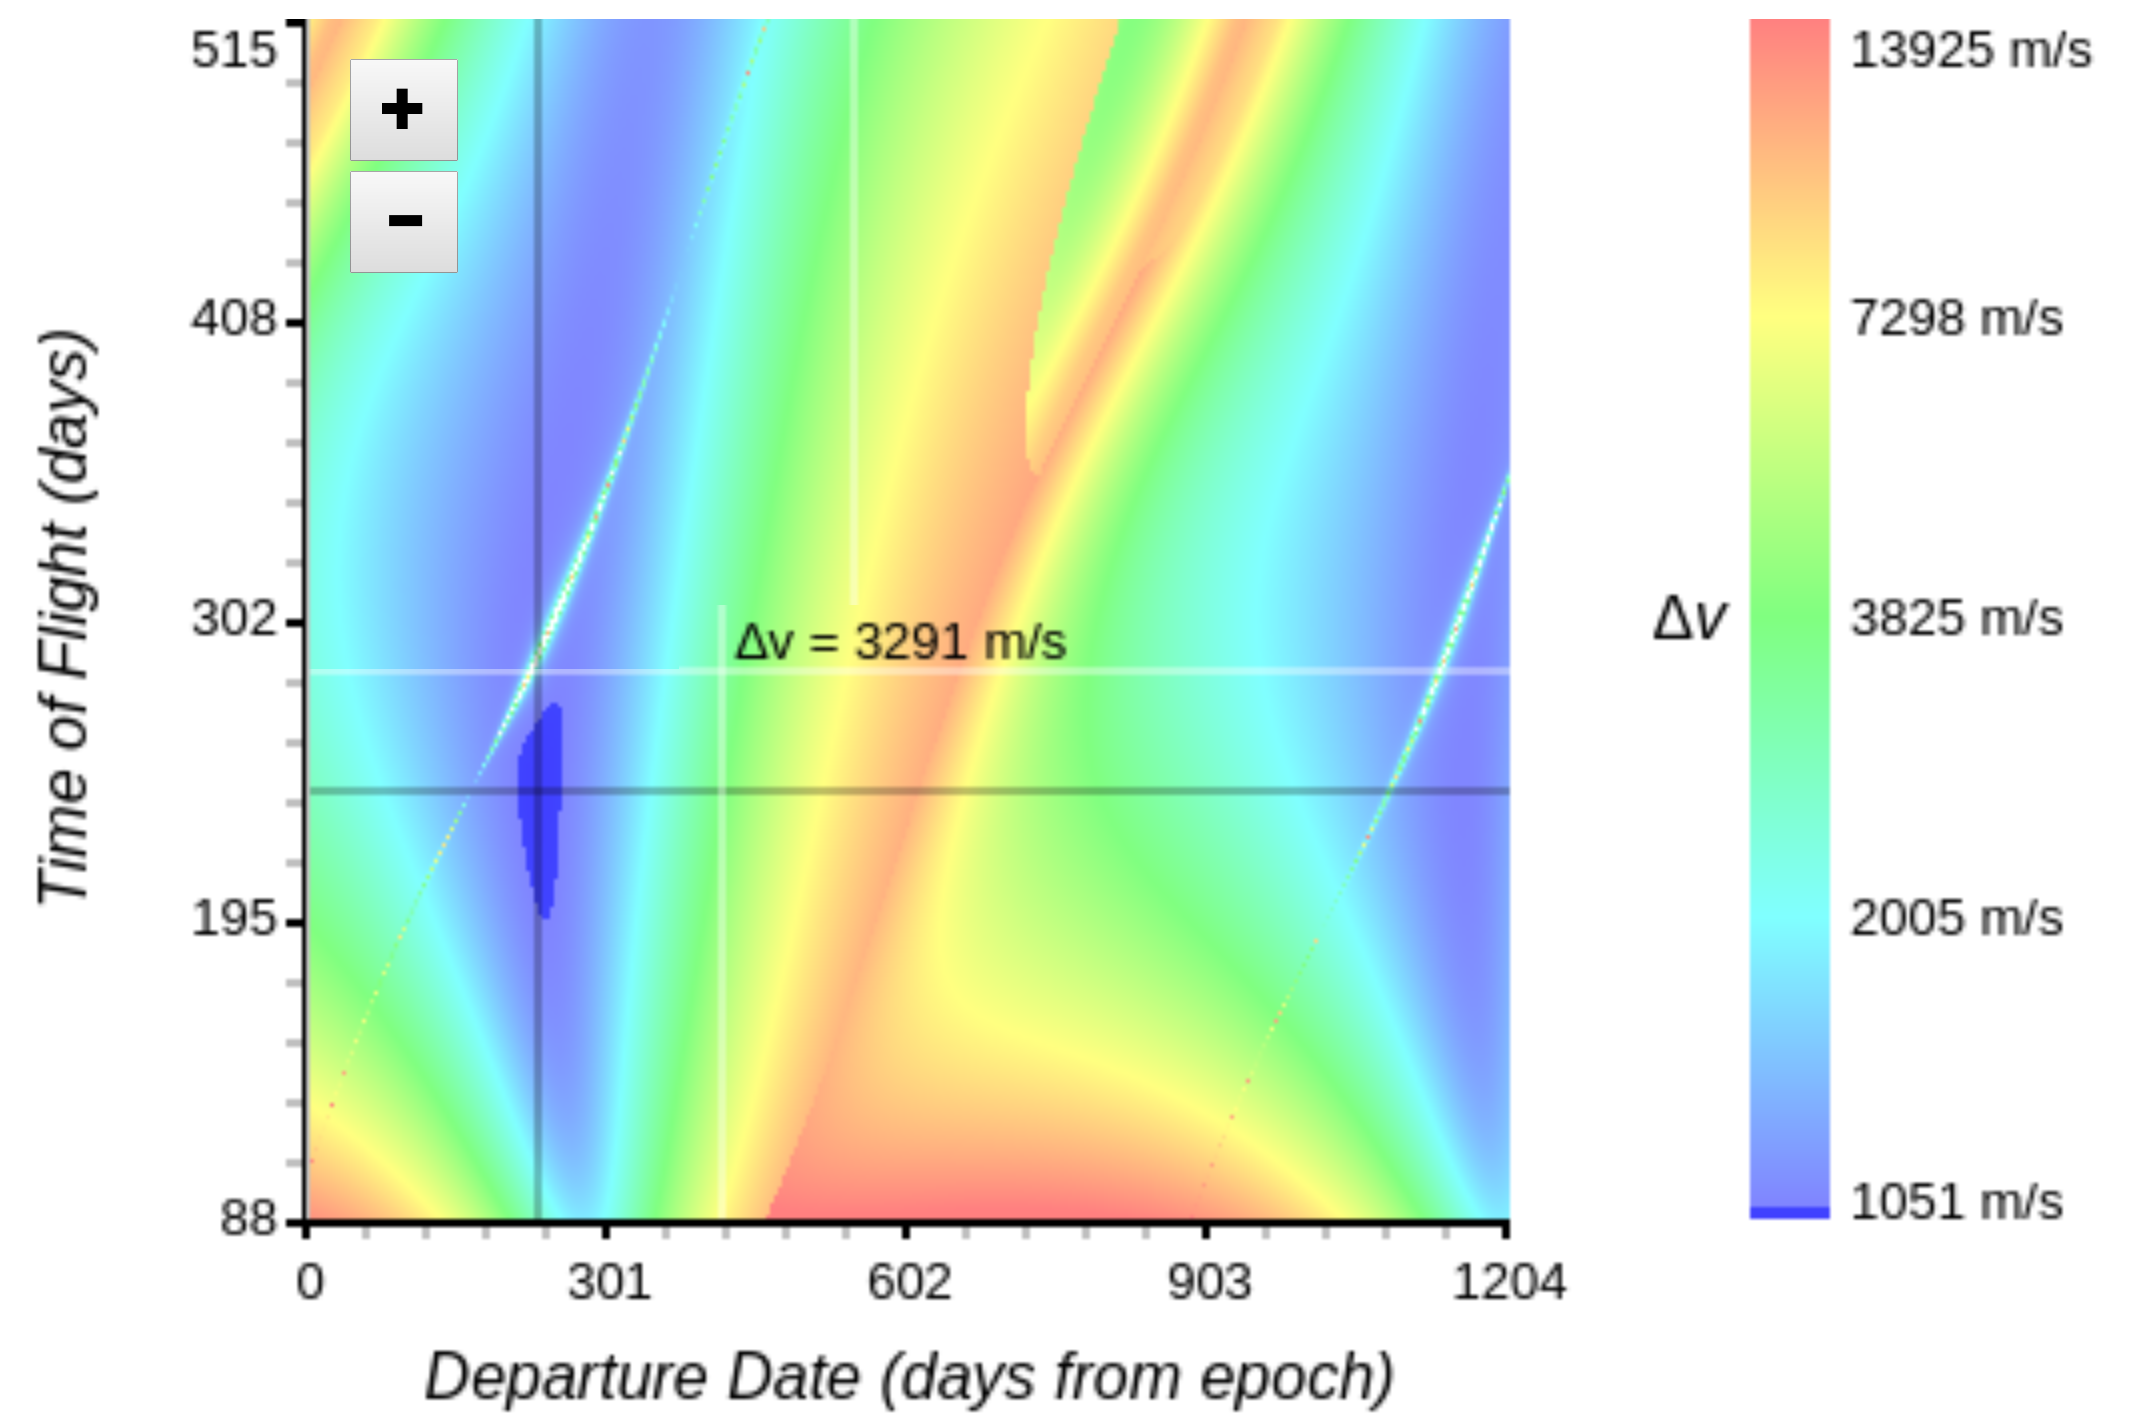
\includegraphics[scale=0.08]{images/hohmann_transfer_window}
        \end{center}
    \end{block}
\end{frame}
{
\usebackgroundtemplate{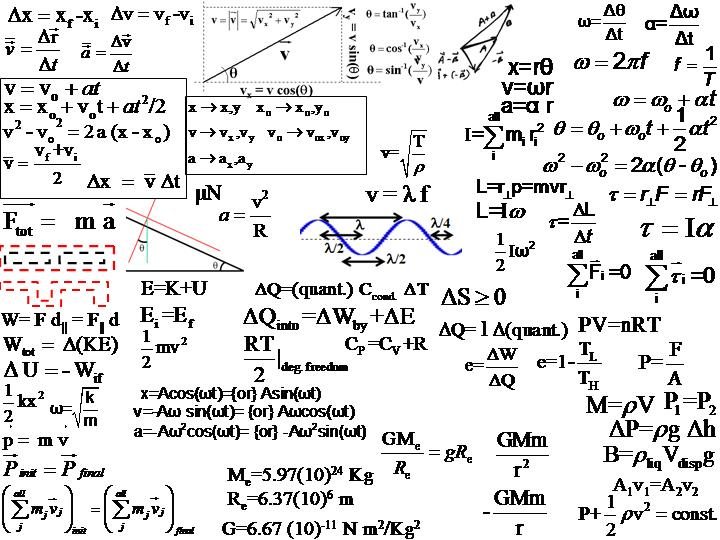
\includegraphics[width=\paperwidth]{images/oberth_troll}}%
\begin{frame}[t]{Oberth effect}
\end{frame}
}
\begin{frame}[t]{jk, Oberth effect}
    \begin{block}{}
        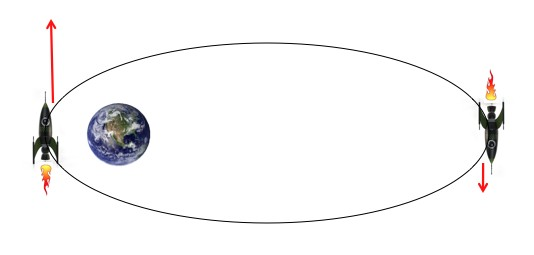
\includegraphics[width=\textwidth]{images/obert_effect}
    \end{block}
\end{frame}
\begin{frame}[t]{Escape}
    \begin{block}{}
        With the Oberth effect we can begin our escape burn and start our transfer orbit
    \end{block}
    \begin{block}{}
        \begin{itemize}
            \item Decelarate to drop orbit deeper into the gravity well
            \item Wait for lowest point of orbit (to make maximal use of Oberth effect)
            \item Make transfer burn and coast to encounter
        \end{itemize}
    \end{block}
\end{frame}

\begin{frame}
    \frametitle{Introduction}
    \begin{block}{}
        \begin{itemize}
            \item We will take you through successfully launching a rocket and landing it on a different body
            \item This is a simplified version based on our vast KSP knowledge
        \end{itemize}
    \end{block}
\end{frame}

\begin{frame}
    \frametitle{Introduction}
    \begin{block}{}
        \begin{itemize}
            \item We will take you through successfully launching a rocket and landing it on a different body
            \item This is a simplified version based on our vast KSP knowledge
        \end{itemize}
    \end{block}
\end{frame}

\begin{frame}
    \frametitle{Introduction}
    \begin{block}{}
        \begin{itemize}
            \item We will take you through successfully launching a rocket and landing it on a different body
            \item This is a simplified version based on our vast KSP knowledge
        \end{itemize}
    \end{block}
\end{frame}


\end{document}
